\documentclass{article}

% Language setting
% Replace `english' with e.g. `spanish' to change the document language
\usepackage[english]{babel}

% Set page size and margins
% Replace `letterpaper' with `a4paper' for UK/EU standard size
\usepackage[letterpaper,top=2cm,bottom=2cm,left=3cm,right=3cm,marginparwidth=1.75cm]{geometry}

% Useful packages
\usepackage{amsmath}
\usepackage{graphicx}
\usepackage{subcaption}
\usepackage[colorlinks=true, allcolors=blue]{hyperref}

\title{\textbf{Do Commodity Prices Grow Faster Than Global Inflation?}}
\author{Chongshuo Zhai
\\Ernest Digore
\\Wei Liu
\\Elliot Beck}

\begin{document}
\maketitle

\begin{abstract}
In this project, we compared the growth of commodity prices, the stock indices, and the inflation rate. It is quite evident that commodities grow faster than inflation and are more volatile. Further, we notice a steady growth in HICP, while commodities experience also periods of extended drawdown. This means that depending on the period chosen, we could actually see inflation growing faster than commodities. Nevertheless, in the long term, commodity prices grow faster. 
\end{abstract}

\section{General View}

\

From the growth rate alone represented in the graphs and tables, it is quite evident that commodities grow faster than inflation and are more volatile. Further, we notice a steady growth in HICP, while commodities experience also periods of extended drawdown. This means that depending on the period chosen, we could actually see inflation growing faster than commodities. Nevertheless, in the long term, commodities grow faster. 

In what follows in this report, we first compose a rather detailed literature review on the related topic and then display and explain some findings from our own research.

\section{Literature Review}

\

Derek Headey and Shenggen Fan in their paper "Anatomy of a crisis: the causes and consequences of surging food prices"~\cite{headey2008anatomy} make an attempt to describe the causes of surging international food prices. They argue that some explanations turn out to hold up much better than others, especially rising oil prices, the depreciation of the U.S. dollar, biofuels demand, and some commodity-specific explanations. A wide range of research has attempted to identify which factors might have caused the surge in food prices (Abbott et al., 2008~\cite{abbott2008s}; Baltzer et al., 2008~\cite{baltzer2008measuring}; Helbling et al., 2008~\cite{helbling2008commodities}; Schnepf, 2008~\cite{schnepf2008high}; Trostle, 2008~\cite{trostle2008fluctuating}; von Braun, 2008~\cite{von2008rising}), and only one paper to date has attempted to add explicit orders of magnitude to different factors (Mitchell, 2008~\cite{mitchell2008note}). This hints, as expected, at the point that commodity prices are interrelated both according to economic theory and empirical data.  

\

Bloch et al. in "Growth, Commodity Prices, Inflation and The Distribution of Income"~\cite{bloch2007growth} specify and estimate a system of equations in which the key dependent variables are world commodity prices, the domestic inflation rate for finished goods and the rate of domestic industrial wage inflation.  Results show that in the short run the primary commodity price index increases by about 1.5 percent for every 1 percent increase in world industrial output, with at most a one-quarter lag. Increases in primary commodity prices on world markets increase costs for manufacturers in all countries, leading to increased finished goods prices. However, their estimates show that the finished goods price increases are always less than proportional. They have measured a short-run elasticity of finished goods price with respect to primary commodity prices of about 0.2 for Japan and the USA, but as low as 0.024 for the UK. The estimates show that rising primary commodity prices stimulate inflation in the industrialized countries as well as raising real incomes of primary producers.

\

In the World Bank's Staff Commodity Working Papers Number 11 - "The Outlook for Primary Commodities, 1984 to 1995"~\cite{duncan1984outlook} it has been mentioned that the prices at that time of non-fuel primary commodities were expected to grow at less than the rate of growth of international inflation. This expectation is based on a continuation of the strict monetary control exercised in industrial countries, no revival of inflationary expectations, and the persistence of excess capacity in the production of the metals/minerals commodities. Again, this entails that the commodity prices are correlated and that inflation is a by-product of developments in the commodity markets where the magnitude takes into consideration also other macroeconomic variables such as exchange rates, yield rates, and inflation expectation. 

\

Ramaprasad Bhar and Anastasios G. Malliaris propose in their paper~\cite{malliaris2011dividends} that the decline in the value of the U.S. dollar, measured both by the appreciation of the Euro and of gold prices, played an important role as oil suppliers demanded compensation for the declining value of the dollar. They also claim that a euphoric stock market represented by the S\&P 500 Index had an impact on oil prices. Using a Markov switching regime methodology they find evidence that this hypothesis is true prior to the financial crisis, but its validity does not hold after the crisis when oil prices crashed along with the S\&P 500 Index. These results once again support the idea that commodity prices are interrelated with each other and that factors such as exchange rate, and volatility in the overall market play a role in influencing the final price. 

\

Another IMF Working Paper developed by Gaston Gelos and Yulia Ustyugova, "Inflation Responses to Commodity Price Shocks – How and Why Do Countries Differ?"~\cite{gelos2012inflation}, relates the inflationary impact of commodity price shocks across countries to a broad range of structural characteristics and policy frameworks over the period 2001–2010, using several approaches. The analysis suggests that economies with higher food shares in CPI baskets, fuel intensities, and pre-existing inflation levels were more prone to experience sustained inflationary effects from commodity price shocks. Countries with more independent central banks and higher governance scores seem to have contained the impact of these shocks better. The effect of the presence of inflation-targeting regimes, however, appears very modest and not evident during the 2008 food price shock. The evidence suggests that trade openness, financial development, dollarization, and labor market flexibility do not significantly influence the way in which domestic inflation responds to international commodity price shocks. Further, countries with higher food shares in their CPI baskets confronted stronger inflationary pressures. However, variables proxying to the importance of fuel in the economy and the CPI were not consistently correlated with the inflationary impact. On the other hand, the energy intensity of the economies in the sample is positively associated with the experienced increase in headline inflation, at least in some specifications. Similarly, to some extent, the inflationary impact was weaker for fuel importers. The transmission to core inflation was stronger for countries with higher CPI inflation levels. Policy variables do not enter significantly the regressions, except for the degree of exchange rate movements, with appreciations of the nominal effective exchange rate associated with a lower impact on core inflation. 

\

Summing up, in the literature it is well recognized that commodity prices affect both headline and core inflation to various extents in terms of magnitude. The degree of pass-through is not trivial to quantify as it depends also on other exogenous variables such as exchange rate, monetary regime, policy implications, weights inside the CPI index, and the stance of the market. Therefore, in our current analysis, we expect that the answer to the question "do commodity prices grow faster than inflation?" will depend on the specifically chosen time interval and the country weights given in the "World Inflation Index" proxy. 

% \

% The table below shows that all the coefficients are statistically significant and explain quite well the variation in inflation (HICP). We can notice that Gold has the highest R2 followed by Cattle. This supports also the idea that gold is a good hedge against inflation by it having a positive coefficient and a high R2. 

\section{Results and Findings}

\subsection{Data Description}

\


We first give a brief introduction to our data. 

\

In this research project, we employed data on the following items:  S\&P 500 Index, Harmonised Index of Consumer Prices (HICP), some classified U.S. inflation data (PCE) from St.Louis Federal Reserve Database, the CRB Commodity Index provided by Bloomberg and some other classified commodity price data from DB$\cdot$NOMICS.

\

The classification of inflation and commodity groups is as follows. Inflation is reported in subgroups of all items, durables, nondurables, services, and core, whereas commodity groups include all, agriculture, food, gold, metal, and oil.

\


\subsection{Figures and Comments}

\

In this subsection we report our main findings accompanied by some visualizing figures.


\begin{figure}[h!]
    \centering
    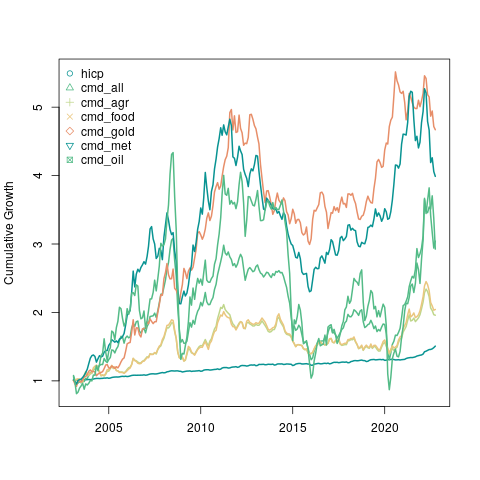
\includegraphics[width=0.5\textwidth]{../../figures/cumgrowth.png}
    \caption{HICP v.s. Commodities}
    \label{fig:cumgrowth}
\end{figure}

\

First, we plotted somewhat brutally, but informatively, Figure~\ref{fig:cumgrowth}, in which one can see the one-line answer to the core question of this project: In the long run, commodity prices do grow faster than inflation. Looking at the figure in more detail, we see that shortly after the start date of this plot, the price of all commodities launched away from the initial price level, with huge volatility, compared to the inflation, which basically grows slowly at a steady pace. 

\

After the year 2005, the overall commodity price only came back to the level of inflation once, due to the dramatic drop of oil price in 2020, but soon grew back to a level that is way higher than the consumption index.

\

However, due to the volatile nature of the commodity prices, we also observe periods of extended drawdown in it. There is not much we can do to compare the two in the short run.

\
\begin{figure}[h!]
    \centering
    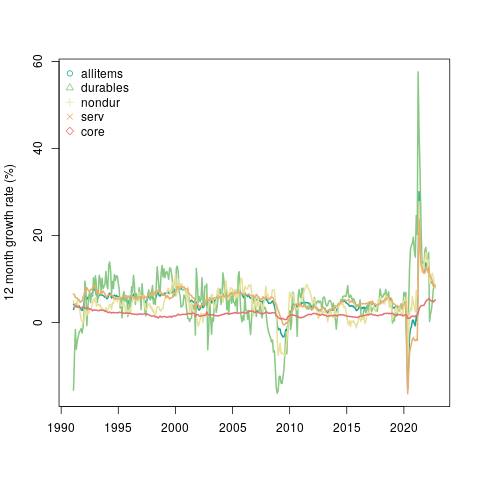
\includegraphics[width=0.5\textwidth]{../../figures/growth12.png}
    \caption{Inflation by Group}
    \label{fig:Inflation_by_group}
\end{figure}

Then we could turn to the Figure~\ref{fig:Inflation_by_group}, which shows the 12-month growth rate of consumption prices in each subclass. We can see that though some groups show volatile price changes, like durables and services, the core inflation and overall inflation (corresponding to the allitems line) are quite stable.

\
\begin{figure}[h!]
    \centering
    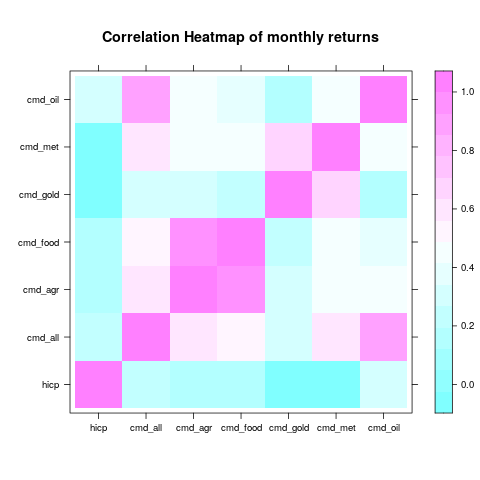
\includegraphics[width=0.5\textwidth]{../../figures/heatmapcmd.png}
    \caption{Correlations between HICP and Commodity Prices}
    \label{fig:heatmapcmd}
\end{figure}

We also explored the correlation between inflation and commodity prices, see Figure~\ref{fig:heatmapcmd}. The first column, showing the correlation between monthly HICP and monthly commodity price changes is of the most interest here. We can see that all blocks showed a positive correlation, though many of them are not too strong. Oil price does correlate the most strongly to inflation, which is consistent with common economic sense. The gold price is almost uncorrelated to the consumption price change, which is again quite explainable since gold is not too relevant to everyday consumption. 

\

There is also some information readable from the rest part of the plot. For example, food prices and agricultural product prices are highly correlated; oil prices contribute the most to the change in overall commodity prices.

\

As is suggested by reference~\cite{malliaris2011dividends}, the stock market, as is demonstrated by S\&P 500, might also interact with both inflation and the commodity market. We also explored this possibility, and made three visualizing plots, as shown in Figure~\ref{fig:SP}.

\ 

The plot Figure~\ref{fig:sfig2} shows a raw picture of how the 12 months returns of the S\&P 500 and CRB commodity index behave. We can see that the pattern the two curves show is quite different before-and-after about 2004. Before that year, there was no immediate consistency seen in the two, while after that year the two curves shared almost every local peak and bottom. 

\

We then turn to look at the correlation heat maps Figure~\ref{fig:sfig1} and \ref{fig:sfig3}. They display the same statistics but on an annual scale and a monthly scale, respectively. In both cases, the stock index showed weak correlations with the commodity index, while in the longer term this interaction was a bit stronger. For the correlation with various classes of inflations, the durables and nondurables are correlated most strongly with the stock market, just the precise ranking of the two is flipped in these two plots. The pattern that the price of durable goods has a larger impact on the stock market in the longer term is again consistent with common economic sense.

\begin{figure}[h!]
\begin{subfigure}{0.33\textwidth}
  \centering
  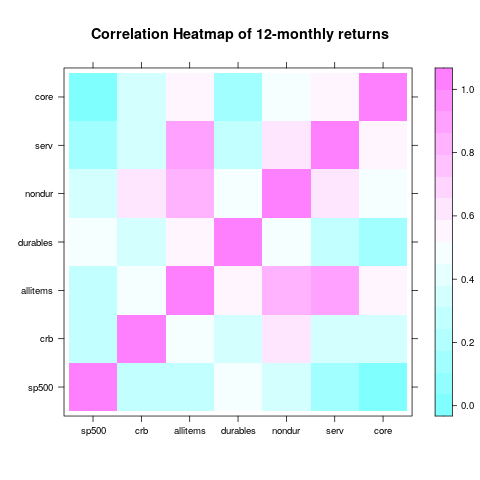
\includegraphics[width=\linewidth]{../../figures/heatmapsp500.png}
  \caption{Correlation between S\&P 500, CRB and Inflations, annually}
  \label{fig:sfig1}
\end{subfigure}%
\begin{subfigure}{0.33\textwidth}
  \centering
  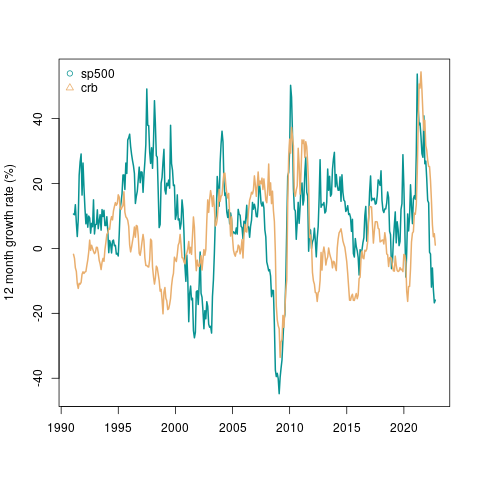
\includegraphics[width=\linewidth]{../../figures/cumgrowth12.png}
  \caption{S\&P 500 v.s. CRB
  \\
   12 months}
  \label{fig:sfig2}
\end{subfigure}
\begin{subfigure}{0.33\textwidth}
  \centering
  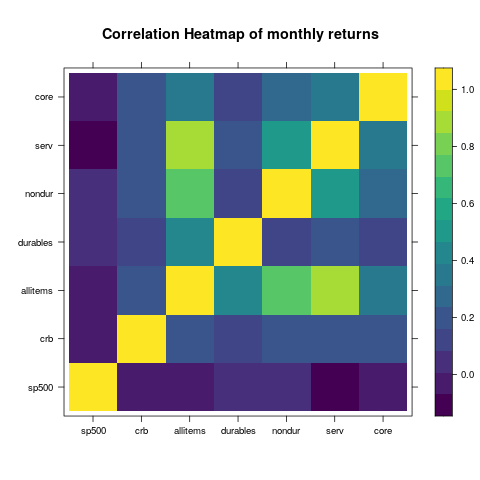
\includegraphics[width=\linewidth]{../../figures/heatmappce.png}
  \caption{Correlation between S\&P 500, CRB and Inflations, monthly}
  \label{fig:sfig3}
\end{subfigure}
\caption{Stock Market, Commodities and Inflation}
\label{fig:SP}
\end{figure}

\section{Conclusions}

To conclude our finding, we first state again the one-liner answer to the core question: The commodity price does grow faster in the long run, but since it's far more volatile, there is no clear conclusion for the short-term comparison.

\

Furthermore, We also found that the inflation on different groups of goods shows different patterns, among which durable goods have the most fluctuating prices, and the "core" products are the most steady.

\

When it comes to the correlation between Commodity prices and inflation, we observed that they are, not too strongly, but positively correlated, and oil price, in particular, shows a slightly stronger correlation with inflation.

\

We also added the stock index to the analysis, as suggested by the literature. We saw that the correlation between the stock index and the  commodity index has become stronger since 2004, but the overall correlation is not too strong. The inflation in the groups of durable and non-durable goods is most strongly correlated to the stock market, and the intensity of the durable class grows as the period of consideration gets longer.

\newpage
\bibliographystyle{plain}
\bibliography{Bibliography}
\end{document}